\documentclass[9pt,a4paper]{extarticle}
\usepackage[T1]{fontenc}
\usepackage{mathptmx}
\usepackage[scaled=0.82]{beramono}
\usepackage[a4paper,left=1.5cm,right=1.5cm,top=1.3cm,bottom=1.3cm]{geometry}
\usepackage{booktabs,tabularx,array,enumitem,titlesec,microtype,amssymb}
\usepackage{tikz}
\usetikzlibrary{arrows.meta,positioning}
\pagestyle{empty}
\setlength{\parindent}{0pt}
\setlength{\parskip}{3pt}
\titleformat{\section}{\large\bfseries}{\thesection}{0.6em}{}
\titlespacing*{\section}{0pt}{7pt}{2pt}
\setlist[itemize]{leftmargin=1.2em,itemsep=0pt,topsep=1pt,parsep=0pt}
\renewcommand{\arraystretch}{1.08}
\newcolumntype{L}{>{\raggedright\arraybackslash}X}
\newcommand{\code}[1]{{\small\texttt{#1}}}

\begin{document}
\textbf{Team No. 14}

\begin{center}
{\Large\bfseries M2: Progress Report}\\[2pt]
Voice-Driven AI Incident Report Assistant (Qualcomm Problem Statement)\\
{\small Target device: Qualcomm QIDK (Snapdragon 8 Elite, Hexagon NPU V79), fully on-device and offline \;$\cdot$\; status at 03:45, 11th October}
\end{center}

\section{Current Approach and Changes since M1}
The approach from M1 is unchanged: tap-to-talk capture $\rightarrow$ on-device Whisper $\rightarrow$ Llama 3.2 3B tool call that fills the form $\rightarrow$ rule-based validator $\rightarrow$ spoken follow-ups for missing mandatory fields only $\rightarrow$ review and submit $\rightarrow$ searchable dashboard. The Android app and the native inference engine are now built and installed on the QIDK. The one part not yet on the board is the Llama NPU bundle, whose export is still running; until it arrives the same engine interface is served by a rule-based fallback extractor, and the app switches to the NPU with a reload and no code change.

\begin{center}\small
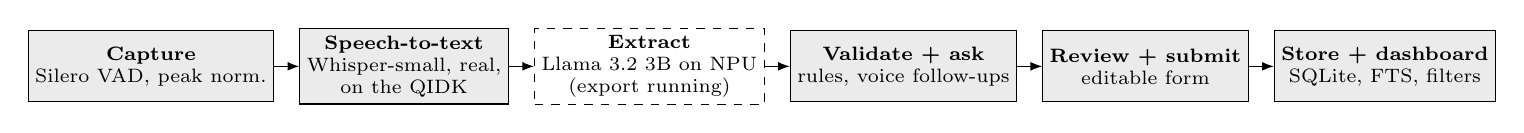
\begin{tikzpicture}[node distance=3.2mm,
  box/.style={draw,align=center,font=\scriptsize,inner sep=2.5pt,minimum height=9mm},
  ok/.style={box,fill=black!8}, wait/.style={box,dashed}]
\node[ok] (a) {\textbf{Capture}\\Silero VAD, peak norm.};
\node[ok,right=of a] (b) {\textbf{Speech-to-text}\\Whisper-small, real,\\on the QIDK};
\node[wait,right=of b] (c) {\textbf{Extract}\\Llama 3.2 3B on NPU\\(export running)};
\node[ok,right=of c] (d) {\textbf{Validate + ask}\\rules, voice follow-ups};
\node[ok,right=of d] (e) {\textbf{Review + submit}\\editable form};
\node[ok,right=of e] (f) {\textbf{Store + dashboard}\\SQLite, FTS, filters};
\foreach \x/\y in {a/b,b/c,c/d,d/e,e/f} \draw[-{Latex[length=1.5mm]}] (\x) -- (\y);
\end{tikzpicture}\\[1pt]
{\scriptsize Shaded: built and running. Dashed: runs through the fallback extractor until the NPU bundle is on the board.}
\end{center}

\begin{tabularx}{\linewidth}{@{}p{2.5cm}p{4.3cm}L@{}}
\toprule
\textbf{Item} & \textbf{Planned at M1} & \textbf{Now, and why}\\
\midrule
Runtime path & Plan A (in-app JNI) or Plan B (shell-user service), to be decided & Plan A chosen. The engine library (JNI, Genie and QNN libraries) is packaged in the APK and loads on Android 15; the app has no internet permission.\\
ASR language & English and Hinglish, automatic detection & Forced English mode. Measured on our 30 clips on the board: automatic detection is about 3$\times$ slower with no gain for English, and Hinglish is weak in every mode (Section 2).\\
ASR robustness & Not planned & Peak normalisation of the recording and a short domain hint for Whisper, added after a live mis-hearing on the board (Section 2).\\
Llama export & Two machines in parallel (laptop and cloud notebook) & Cloud notebook dropped: it has 31\,GB RAM without swap and the export ran out of memory. The laptop export continues, with a patched uploader and resume so finished parts are never re-sent.\\
Search & SQLite FTS5 & Room FTS4 (available without bundling a separate SQLite); prefix search with snippets works.\\
Recommendations & SOP list, LLM tailoring later & SOP templates only for the demo; no extra model call.\\
Scope cuts & -- & Draft-resume screen, charts, PDF/JSON export and narrations above 30\,s are left out to protect the core flow.\\
\bottomrule
\end{tabularx}

\section{Experiments Run So Far and Results}
\begin{tabularx}{\linewidth}{@{}p{3.3cm}p{5.2cm}L@{}}
\toprule
\textbf{Experiment} & \textbf{Setup} & \textbf{Result}\\
\midrule
ASR accuracy, on device & Whisper-small (q5\_1, whisper.cpp, CPU) on the QIDK, 30 recorded clips, three language modes & English mode: \textbf{WER 7.0\,\%}, about 1.9\,s per clip. Automatic mode: about 3$\times$ slower, no English gain. Hinglish: CER about 70\,\% in every mode.\\
ASR speed, on device & 11\,s reference clip, before and after tuning the native decoder settings & 3.4\,s $\rightarrow$ \textbf{1.45\,s} (about 7.5$\times$ faster than real time).\\
ASR, live recording & Spoken slide example on the board microphone, SNR about 11\,dB & ``water leak'' was heard as ``virtual leap''. With a short domain hint the same audio is transcribed correctly offline; the hint is written by the app and a patch for the native engine is ready.\\
Extraction, first run (preliminary) & Stock Llama 3.2 3B, 4-bit, on a laptop GPU (not the NPU), first prompt version, 150-case text set; the run was interrupted and is being repeated & Incident type \textbf{81.0\,\%} (target 90). Per-field F1 micro \textbf{0.611} (P 0.565, R 0.666), macro 0.409 (target 0.80). Mapping accuracy \textbf{83.1\,\%} (target 95). Below target, so prompt work is in progress.\\
Pipeline correctness without the model & The 150 expected tool calls passed through parser $\rightarrow$ merger $\rightarrow$ time resolver $\rightarrow$ validator & 150/150 accepted with no field dropped. Follow-up question equals the expected one in 39/50 cases; the other 11 differ because a severity rule already fills the field.\\
Two implementations compared & App-side and ML-side time resolver, location matcher and prompt builder & Prompts identical byte for byte; time resolver identical on every phrase in the set; location matcher differs only for bare ``Block A/B''.\\
Export upload & Model parts to AI Hub over a mobile hotspot & One connection gives about 30\,kB/s; 48 parallel connections give about 2.5\,MB/s. First part (820\,MB) uploaded in about 5 minutes.\\
\bottomrule
\end{tabularx}

\textbf{What the results changed.} The ASR numbers decided the language mode. The live mis-hearing showed that clean-clip WER is not enough, which led to normalisation and the domain hint. The first extraction run shows the stock model with the first prompt is not yet at target; the errors are mostly extra fields (precision 0.565), which the grounding check and schema validator in the app already remove before the form is shown, so the next run will also be scored after that step. Hinglish speech is the weakest part: it works end to end but with lower accuracy, and we will state this openly in the demo.

\section{Progress on Testing}
\begin{itemize}
\item \textbf{Test data (done):} 150 template-generated text cases over all 10 categories (complete reports, missing fields, self-corrections, filler words, relative times, Hinglish), each with the expected value for every field and the expected follow-up; 30 recorded audio clips with reference transcripts. The dev split (42 cases) was fixed before prompt tuning.
\item \textbf{Automated tests (done): 321 passing.} 190 in the shared core (validator, parser, normalisers, prompt builder), 119 in the app domain layer (conversation state machine including the full slide example, time resolver, location matcher, form merger) and 12 in the app (database and full-text search on a real SQLite).
\item \textbf{App run on Android 15 arm64 (done):} every screen exercised on an emulator: capture with VAD timeout, conversation, review with the submit gate, dashboard search and filters, detail and edit, emergency banner and dialler. Eight defects were found only by running the app and are fixed, for example a wrong reference-number format, the keyboard covering the input field, and seed data that failed the validator.
\item \textbf{On the QIDK (in progress):} app installed and launching; Whisper model and Hexagon V79 libraries on the board; real speech-to-text working; eSpeak set as the voice. The on-device evaluation runner is written; it has produced the ASR results and will produce the extraction results once the bundle is loaded.
\item \textbf{Not done yet:} extraction accuracy on the NPU, the rules-only baseline comparison, per-stage latency (p50/p90), tokens per second, temperature, and the run of 20 consecutive spoken reports.
\end{itemize}

\section{Plan for the Remaining Time}
\begin{tabularx}{\linewidth}{@{}p{2.2cm}L@{}}
\toprule
\textbf{Time} & \textbf{Work}\\
\midrule
04:00--05:30 & Finish the Llama 3.2 3B V79 export; push the bundle to the board; NPU smoke test; reload the app onto the NPU. In parallel: prompt fixes on the dev split, apply the ASR domain-hint patch, microphone and VAD thresholds with real noise.\\
05:30--07:30 & On-device evaluation through the real pipeline: extraction and mapping accuracy on the held-out cases, rules-only baseline, latency per stage and tokens per second. Fix the largest error groups.\\
07:30--09:00 & 20 consecutive spoken reports on the board in airplane mode; check stability and temperature; freeze the build.\\
09:00--11:00 & Final report, README, licence, demo video, code zip; slides by 11:30.\\
\bottomrule
\end{tabularx}

\textbf{Risks and fallbacks.} If the 3B bundle is not on the board by about 05:30 we export Llama 3.2 1B (a much smaller upload), and if that also fails we run a quantised model with llama.cpp on the CPU behind the same engine interface. The app does not depend on which of these is used. If prompt changes do not reach the extraction targets, we report the measured numbers together with the baseline rather than tuning on the held-out set.

\end{document}
